\documentclass[a4paper,10pt]{article}

\usepackage[margin=22mm]{geometry}
\usepackage{amsmath,amssymb}
\usepackage{booktabs}
\usepackage{float}
\usepackage{graphicx}
\usepackage{microtype}
\usepackage{natbib}
\usepackage{tikz}
\usepackage{xcolor}
\usepackage{hyperref}
\usepackage{listings}
\usetikzlibrary{positioning}

\hypersetup{
  colorlinks=true,
  linkcolor=blue!55!black,
  citecolor=blue!55!black,
  urlcolor=blue!55!black,
  pdftitle={GPU SPH with Massively: Expressing Dynamic Neighborhoods with Cell Graphs and Nested Segmented Iterators},
  pdfauthor={Akira Hayakawa},
  pdfsubject={Implementation challenges of GPU SPH and their solution in Massively v0.80}
}
\graphicspath{{../workspace/plot/}}
\newcommand{\code}[1]{\texttt{#1}}
\newcommand{\Seg}{\operatorname{Seg}}
\newcommand{\Perm}{\operatorname{Permute}}
\lstset{
  basicstyle=\ttfamily\small,
  frame=single,
  columns=fullflexible,
  keepspaces=true,
  breaklines=true,
  showstringspaces=false
}

\title{GPU Smoothed Particle Hydrodynamics with Massively:\\
Expressing Dynamic Neighborhoods with Cell Graphs\\
and Nested Segmented Iterators}
\author{Akira Hayakawa}
\date{July 18, 2026}

\begin{document}
\maketitle

\begin{abstract}
The principal implementation difficulty in GPU Smoothed Particle Hydrodynamics
(SPH) is not the pair formula itself but its moving, variable-length
neighborhood.  This paper explains how that workload is expressed using the
iterator algebra of Massively v0.80.  A uniform-grid cell adjacency is stored
once as a compressed sparse row (CSR) graph.  At each derivative evaluation,
particle state is sorted by cell and lower bounds form a second CSR partition
from cells to particles.  Lazy permutation and two nested
\code{SegmentIterator} values then compose both structures into one
segment-of-segments per query particle.  A \code{Segment} is a read-only semantic
view whose GPU value contains bounds rather than copied neighbor data; thus no
global particle-pair list is materialized.  One transform invocation owns one
query particle and gathers all contributions into private accumulators, avoiding
atomics and write conflicts.  We also report how the solver is decomposed to
respect Massively's type-level limit of 13 read leaves.  The Sod shock tube is
used as the end-to-end physical check and gives a sampled density $L_1$ error of
0.004199 at $t=0.15$.  GPU density agrees with a CPU all-pairs reference to a
maximum relative difference of $5.89\times10^{-6}$ at 65,536 particles.  On an
integrated Radeon 680M, the complete two-dimensional density snapshot takes
5.109 ms, compared with 16.204 ms for a CPU cell-list calculation.  The result
is an implementation study: it identifies the obstacles in mapping SPH to a
typed GPU iterator system, shows the corresponding Massively construction, and
measures its costs and benefits without proposing a new SPH discretization.
\end{abstract}

\section{Introduction}

Smoothed Particle Hydrodynamics replaces an Eulerian mesh by moving particles
and compactly supported interpolation kernels \citep{gingold1977,monaghan1992}.
For particle $i$, density, pressure force, and artificial viscosity are sums over
nearby particles.  The numerical formula is naturally parallel over $i$, but
the set of contributing particles changes whenever the particles move.  A GPU
implementation must therefore repeatedly turn positions into a ragged
neighborhood relation while preserving coalesced state access and bounded
memory use.

Conventional GPU SPH implementations solve this problem with sorted cell lists,
linked cells, Verlet lists, or explicit interaction kernels
\citep{herault2010,dominguez2011,dominguez2013,winkler2018}.  Massively takes a
different programming route.  It supplies device algorithms and a typed algebra
of logical iterators on CubeCL \citep{massively080,cubecl}.  Operations such as
zip, transform, permutation, and segmentation can be composed before an
executing algorithm lowers the expression to a GPU kernel.  The question in
this work is consequently precise:

\begin{quote}
How can a moving SPH neighborhood be represented as Massively iterators without
allocating one stored neighbor list per particle, and how should the remaining
GPU constraints be handled in a complete solver?
\end{quote}

The contributions of this paper are:
\begin{itemize}
  \item an explicit derivation of the SPH neighborhood as the composition of a
        static cell CSR, a dynamically rebuilt cell--particle partition, lazy
        permutation, and nested segmented iteration;
  \item a race-free gather formulation in which each GPU invocation evaluates
        one query particle and writes one output, including its memory and work
        trade-offs;
  \item a field-by-field decomposition of one- and two-dimensional density,
        pressure, work, and viscosity kernels under Massively v0.80's 13-read
        type-level arity bound; and
  \item evidence from structural and differential tests, the Sod shock tube,
        and a density-pipeline benchmark.
\end{itemize}

The implementation uses a fixed smoothing length, the cubic spline,
first-order time integration, and artificial viscosity.  Its end-to-end
physical validation is the standard Sod shock tube.

\section{The implementation problem posed by SPH}

\subsection{The pairwise workload}

For particle position $\mathbf{x}_i$, velocity $\mathbf{v}_i$, mass $m_i$,
density $\rho_i$, specific internal energy $e_i$, and smoothing length $h$, the
implemented density estimate is
\begin{equation}
  \rho_i = \sum_j m_j W_d(\lVert\mathbf{x}_i-\mathbf{x}_j\rVert,h).
  \label{eq:density}
\end{equation}
The ideal-gas equation of state is $p_i=(\gamma-1)\rho_i e_i$.  Pressure and
viscous derivatives have the generic SPH form
\begin{align}
  \frac{d\mathbf{v}_i}{dt}
    &= -\sum_j m_j\left(\frac{p_i}{\rho_i^2}
                       +\frac{p_j}{\rho_j^2}+\Pi_{ij}\right)
       \nabla_i W_{ij}, \\
  \frac{de_i}{dt}
    &= \sum_j m_j\frac{p_i}{\rho_i^2}
       (\mathbf{v}_i-\mathbf{v}_j)\mathbin{\cdot}\nabla_iW_{ij}
       +\frac12\sum_jm_j\Pi_{ij}
       (\mathbf{v}_i-\mathbf{v}_j)\mathbin{\cdot}\nabla_iW_{ij}.
  \label{eq:derivatives}
\end{align}
These equations are standard conservative SPH forms
\citep{monaghan2005,price2012}.  The implementation uses the cubic B-spline
\begin{equation}
 W_d(r,h)=\frac{\sigma_d}{h^d}
 \begin{cases}
  1-\tfrac32q^2+\tfrac34q^3,&0\le q<1,\\
  \tfrac14(2-q)^3,&1\le q<2,\\
  0,&q\ge2,
 \end{cases}
 \qquad q=r/h,
 \label{eq:kernel}
\end{equation}
where $\sigma_1=2/3$ and $\sigma_2=10/(7\pi)$.  Hence a pair contributes only
when $r<2h$.

Artificial viscosity is evaluated only for approaching particles.  In
dimensionless coordinates $\mathbf{q}_{ij}=(\mathbf{x}_i-\mathbf{x}_j)/h$, the
implementation has the coefficient form
\begin{equation}
 \mu_{ij}=\frac{(\mathbf{v}_i-\mathbf{v}_j)\cdot\mathbf{q}_{ij}}
                 {\lVert\mathbf{q}_{ij}\rVert^2+0.01},\qquad
 \Pi_{ij}=\frac{-A\mu_{ij}+B\mu_{ij}^2}{\widehat\rho_{ij}}.
 \label{eq:viscosity}
\end{equation}
The one-dimensional coefficients are configurable and use an arithmetic mean
density.  The current two-dimensional workload uses $A=1$, $B=2$, and
$\widehat\rho_{ij}=\sqrt{\rho_i\rho_j}$.  This numerical choice is not the
contribution of the paper; its factorization is relevant later because it makes
the operation expressible within Massively's read-arity bound.

Equations~\eqref{eq:density}--\eqref{eq:derivatives} expose the GPU workload.
Each output particle has a different number of candidate neighbors; a candidate
requires several query and neighbor columns; and the same spatial relation is
reused for density, pressure, and viscosity with different column tuples.

\subsection{Five mapping obligations}

The implementation must satisfy five obligations simultaneously:
\begin{enumerate}
  \item \textbf{Complete dynamic neighborhoods.}  Every pair inside support
        must be visited after arbitrary particle motion, without an $O(N^2)$
        scan.
  \item \textbf{Coherent reordering.}  Sorting position but not velocity, mass,
        energy, and particle identity would silently mix different particles.
  \item \textbf{Race-free accumulation.}  A symmetric pair operation tempts an
        implementation to update both $i$ and $j$, which requires atomics or a
        coloring scheme on a GPU.
  \item \textbf{Bounded representation.}  Materializing all candidate pairs
        adds memory proportional to the sum of per-particle candidate counts and
        must be rebuilt as particles move.
  \item \textbf{Expressible kernels.}  The composed input must fit the static
        iterator types and kernel read-arity supported by Massively v0.80.
\end{enumerate}
Keeping particle data on the device is an additional practical requirement:
otherwise a correct neighborhood kernel can be dominated by transfers at every
time step.

\section{Massively mechanisms used by the solver}

\subsection{Logical iterators and execution points}

Massively distinguishes logical input expressions from algorithms that allocate
and execute.  A slice of a device vector is an iterator; \code{zip} combines
columns, \code{lazy::transform} changes the value read at an index, and
\code{lazy::permute(values, indices)} reads \code{values[indices[i]]}.  These
expressions do not by themselves create result arrays.  An operation such as
\code{vector::transform}, \code{vector::sort\_by\_key}, or
\code{vector::lower\_bound} is an execution point that produces device storage.

This separation is central to the design.  The solver materializes the data that
must change globally---sorted particle columns, cell identifiers, cell offsets,
and physical outputs---while representing the relation between those arrays as
lazy readers.

\subsection{What a SegmentIterator represents}

Given a logical value stream $V$ and offsets
$P=(P_0,\ldots,P_K)$, Massively defines
\begin{equation}
 \Seg(V,P)[k] = V[P_k:P_{k+1}).
 \label{eq:segment}
\end{equation}
The item type of the resulting \code{SegmentIterator} is
\code{Segment<V::Item>}.  A \code{Segment} is not an owned vector and has no
allocation or write capability.  Its generated GPU value varies only by the
\code{start} and \code{len} bounds held in registers; the backing reader is
compiler-side context shared by the segments of that expression.  Inside a
CubeCL operation, \code{len()} returns the dynamic length and \code{at(k)} emits
a read of the backing expression at \code{start + k}.

Two consequences matter for SPH.  First, segments may be permuted without
copying their particle data.  Second, the values of one segment iterator may
themselves be segments, yielding an outer \code{Segment} whose item is an inner
\code{Segment<ParticleFields>}.  This is precisely the type required to express
``the neighboring cells, and the particles in each neighboring cell.''

\subsection{The read-arity boundary}

Massively assigns a type-level read arity to a canonical input expression.  In
v0.80 the available arities are $A_1,\ldots,A_{13}$, and type-level addition is
defined only when the total is at most 13.  This catches oversized compositions
at compile time, but also means that a physically natural all-in-one SPH
expression may not be representable.  Section~\ref{sec:whole-solver} shows how
the implementation splits such expressions while preserving the same
neighborhood view.

\section{Constructing a moving neighborhood}

\subsection{Static cell graph}

Let the cell width be $s=2h$, equal to the compact support radius.  In one
dimension each cell is adjacent to itself and at most two neighboring cells; in
two dimensions it is adjacent to the $3\times3$ block clipped at the domain
boundary.  This relation depends on the domain geometry but not on particle
positions, so it is built once as CSR:
\begin{align}
 A &= (A_0,\ldots,A_{E-1}) &&\text{neighbor cell identifiers},\\
 G &= (G_0,\ldots,G_C) &&\text{row offsets},\\
 \mathcal{G}(c) &= A[G_c:G_{c+1}).
\end{align}
For $C$ cells, $E\le3C$ in one dimension and $E\le9C$ in two dimensions.

The graph is complete for the kernel support.  If
$\lVert\mathbf{x}_i-\mathbf{x}_j\rVert<2h=s$, the absolute displacement in each
coordinate is less than $s$.  The integer cell coordinates can therefore differ
by at most one in each dimension.  The CSR row enumerates every such cell offset.
Candidates in the corner of a two-dimensional $3\times3$ block but outside the
circular support are rejected by Equation~\eqref{eq:kernel} inside the pair loop.

\subsection{Dynamic cell--particle partition}

At every derivative evaluation, a Massively \code{vector::transform} maps each
position to a clamped row-major cell identifier $c_i$.  The implementation then
performs one \code{sort\_by\_key} whose value is the complete zipped
structure-of-arrays state.  In one dimension this tuple has eight fields; in two
dimensions it has ten.  Sorting the tuple once maintains the invariant
\begin{equation}
  (\mathrm{id},\mathbf{x},\mathbf{v},e,m,\text{precomputed mass factors})_k
  \quad\text{all belong to the same particle.}
\end{equation}
The sorted cell key is retained alongside the reordered state.

For every cell identifier $0,\ldots,C$, \code{vector::lower\_bound} searches the
sorted keys.  Its output
$P=(P_0,\ldots,P_C)$ partitions the particle stream:
\begin{equation}
 \mathcal{B}(c)=V[P_c:P_{c+1}).
 \label{eq:cell-particles}
\end{equation}
An empty cell needs no special case: it simply has $P_c=P_{c+1}$.

\subsection{Composition into nested segments}

The central construction can now be stated independently of Rust types.  Let
$V$ be any zipped neighbor-field stream in sorted particle order.  Define
\begin{align}
 B &= \Seg(V,P),
   & B[c] &= \mathcal{B}(c),\\
 R &= \Perm(B,A),
   & R[e] &= B[A_e],\\
 H &= \Seg(R,G),
   & H[c] &= (B[A_{G_c}],\ldots,B[A_{G_{c+1}-1}]),\\
 N &= \Perm(H,c),
   & N[i] &= H[c_i].
 \label{eq:nested}
\end{align}
Thus $N[i]$ is a segment of cell segments for query particle $i$.  The exact
Massively pattern, with type conversions omitted, is shown in
Listing~\ref{lst:nested}.

\begin{lstlisting}[caption={Schematic Massively construction of one SPH neighborhood view.},label={lst:nested}]
let b = SegmentIterator::new(values, particle_offsets);
let r = lazy::permute(b, neighbor_cells);
let h = SegmentIterator::new(r, graph_offsets);
let n = lazy::permute(h, cell_ids);
let output = vector::transform(exec, zip(query, n), PairReduction)?;
\end{lstlisting}

The first \code{SegmentIterator} is backed by the materialized sorted columns and
particle offsets.  The permutation by $A$, the second segmentation by $G$, and
the final permutation by $c_i$ remain logical read expressions.  In particular,
there is no array containing all $(i,j)$ pairs and no array containing a copied
neighbor vector for each $i$.  The physical topology inputs of the nested view
are only $P$, $A$, $G$, and $c$.

\begin{figure}[H]
  \centering
  \resizebox{\textwidth}{!}{%
  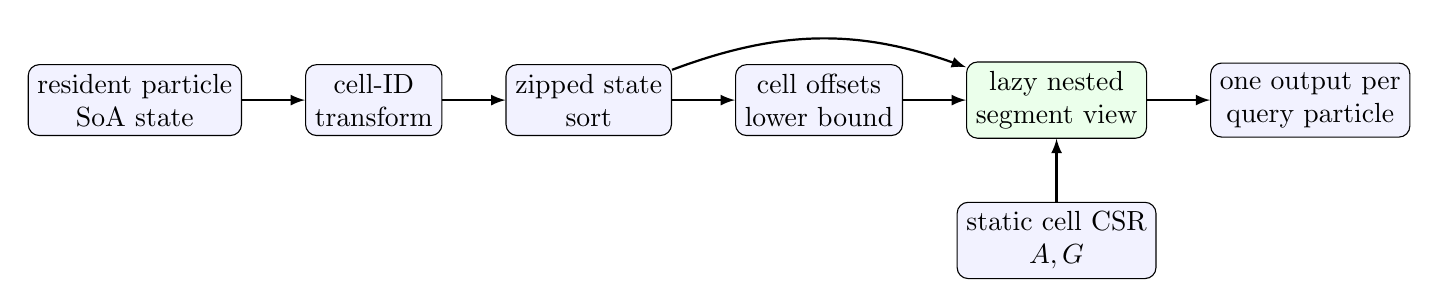
\begin{tikzpicture}[
      node distance=8mm and 8mm,
      box/.style={draw,rounded corners,align=center,minimum height=9mm,fill=blue!5},
      view/.style={draw,rounded corners,align=center,minimum height=9mm,fill=green!8},
      arrow/.style={-latex,thick}]
    \node[box] (state) {resident particle\\SoA state};
    \node[box,right=of state] (key) {cell-ID\\transform};
    \node[box,right=of key] (sort) {zipped state\\sort};
    \node[box,right=of sort] (offset) {cell offsets\\lower bound};
    \node[view,right=of offset] (nested) {lazy nested\\segment view};
    \node[box,right=of nested] (reduce) {one output per\\query particle};
    \node[box,below=of nested] (graph) {static cell CSR\\$A,G$};
    \draw[arrow] (state)--(key);
    \draw[arrow] (key)--(sort);
    \draw[arrow] (sort)--(offset);
    \draw[arrow] (offset)--(nested);
    \draw[arrow] (sort) to[bend left=20] (nested);
    \draw[arrow] (graph)--(nested);
    \draw[arrow] (nested)--(reduce);
  \end{tikzpicture}}
  \caption{Materialized stages are blue; the green nested neighborhood is a
  lazy view.  Rebuilding membership does not rebuild the static cell graph.}
  \label{fig:neighborhood}
\end{figure}

\subsection{Race-free gather and cost}

The final \code{vector::transform} launches one logical operation per query
particle.  That operation traverses the outer cell segment and the inner
particle segment, rejects $q\ge2$, and accumulates into operation-local CubeCL
\code{RuntimeCell} values.  Invocation $i$ writes only output $i$.  No invocation
writes a neighbor's derivative, so no atomic addition or pair coloring is
required.

The trade-off is intentional: an interacting unordered pair is normally
evaluated twice, once as $i\mathbin{\to}j$ and once as
$j\mathbin{\to}i$.  A scatter formulation could reuse the pair arithmetic but
would reintroduce synchronization.  The gather formulation instead favors a
simple ownership rule and contiguous query outputs.

Let $Q$ be the number of ordered candidate interactions enumerated by the cell
rows.  The stored representation is $O(N+C+E)$, whereas a persistent candidate
list is $O(N+Q)$.  One preparation has the work model
\begin{equation}
 T_{\mathrm{prepare}}=
 T_{\mathrm{sort}}(N)+O(N)+O(C\log N)+O(Q),
 \label{eq:cost}
\end{equation}
where $T_{\mathrm{sort}}$ is left backend-dependent and $C+1$ lower-bound
queries account for the $O(C\log N)$ term.  If cell occupancy remains bounded,
$Q=O(N)$.  This analysis does not remove divergence caused by unequal segment
lengths; Massively supplies the representation and lowering mechanism, while
the physical particle distribution still controls the executed work.

\section{Mapping the complete solver}
\label{sec:whole-solver}

\subsection{Device-resident pipeline}

Particle identity, position, velocity, internal energy, mass, and powers of
$m/h$ are uploaded into structure-of-arrays device vectors.  One step executes
the following stages:
\begin{enumerate}
  \item compute cell identifiers, sort the complete zipped state, and obtain
        particle offsets;
  \item scale positions by $h^{-1}$ and evaluate density through the nested
        neighborhood;
  \item evaluate the ideal-gas equation of state elementwise;
  \item rebuild typed views over the same sorted particles for pressure, pressure
        work, and viscosity, then evaluate their pair reductions;
  \item combine derivatives and update energy, velocity, and position; and
  \item retain the new arrays on the device for the next step.
\end{enumerate}
Only \code{snapshot} performs explicit device-to-host transfer.  Sorting changes
storage order, so snapshots carry stable particle identifiers; physical output
can be restored to identity order off-device when required.

The neighborhood is rebuilt as a typed view for each physical operator because
the required neighbor tuple differs.  Density reads position and a mass factor;
pressure additionally reads $p/\rho^2$; viscosity reads velocities and density
factors.  These views share the already materialized $P$, $A$, $G$, and $c$.

\subsection{Working within 13 read leaves}

Table~\ref{tab:arity} counts the physical leaves in each composed input.  The
four topology leaves are the particle offsets $P$, neighbor-cell identifiers
$A$, cell-graph row offsets $G$, and query cell identifiers $c$.  Query and
neighbor columns make up the remainder.

\begin{table}[ht]
  \centering
  \caption{Read-arity decomposition in Massively v0.80.}
  \label{tab:arity}
  \begin{tabular}{lrrrr}
    \toprule
    Operation & query fields & neighbor fields & topology & total \\
    \midrule
    1-D density                  & 1 & 2 & 4 & 7 \\
    2-D density                  & 2 & 3 & 4 & 9 \\
    1-D pressure derivative      & 3 & 4 & 4 & 11 \\
    1-D viscosity derivative     & 5 & 4 & 4 & 13 \\
    2-D pressure acceleration    & 3 & 4 & 4 & 11 \\
    2-D pressure work, per axis  & 4 & 4 & 4 & 12 \\
    2-D viscosity derivative     & 4 & 5 & 4 & 13 \\
    \bottomrule
  \end{tabular}
\end{table}

The one-dimensional viscosity expression reaches the limit exactly.  In two
dimensions, pressure acceleration is evaluated in one pass, while pressure work
is split into $x$ and $y$ passes.  Attempting to zip both velocity components and
all pressure data into one neighborhood expression would exceed the available
type-level arity.

Two-dimensional viscosity requires positions, both velocity components, a mass
gradient factor, and density.  The implementation first materializes
\begin{equation}
 f_j=\frac{m_j}{h^3\sqrt{\rho_j}},
\end{equation}
uses $f_j$ as one neighbor field in the 13-leaf pair pass, and multiplies the
three resulting derivatives by $1/\sqrt{\rho_i}$ in an elementwise post-pass.
This realizes the geometric mean in Equation~\eqref{eq:viscosity}.  The split
costs two additional dispatches and intermediate arrays, but it illustrates a
general Massively technique: move separable per-particle factors outside a
ragged pair reduction when the combined expression is too wide.

\subsection{Challenge-to-mechanism summary}

\begin{table}[ht]
  \centering
  \caption{How the SPH implementation obligations map to Massively.}
  \label{tab:solutions}
  \begin{tabular}{p{0.21\textwidth}p{0.40\textwidth}p{0.27\textwidth}}
    \toprule
    SPH/GPU problem & Massively realization & Residual cost or trade-off \\
    \midrule
    Moving, ragged neighborhood
      & Cell-ID transform, zipped sort, lower bounds, then nested
        \code{SegmentIterator} views
      & Sort and offsets are rebuilt for each derivative evaluation \\
    Candidate-list memory
      & Lazy permutation composes cell and particle CSR without copying pair data
      & Candidate arithmetic is still performed at traversal time \\
    Parallel write conflicts
      & One transform invocation gathers one query particle into private state
      & Symmetric unordered pairs are generally evaluated twice \\
    SoA column alignment
      & One tuple is the value of \code{sort\_by\_key}; all columns move together
      & Every persistent field must be included in that tuple \\
    Wide physical operator
      & Per-axis passes and separable pre/post transforms satisfy $A_{13}$
      & Extra dispatches and temporary device vectors \\
    Repeated host transfer
      & Executing algorithms produce resident device vectors; snapshots are explicit
      & Host inspection remains a synchronization point \\
    \bottomrule
  \end{tabular}
\end{table}

\section{Validation and evaluation}

\subsection{Implementation-level checks}

The tests are layered around failure modes of the mapping rather than around a
large collection of hydrodynamic benchmarks.  Deterministic and
\code{proptest}-generated cases check cubic-spline compact support and symmetry,
CSR row uniqueness and symmetry, expected boundary/interior row degrees, and
the neighborhood completeness condition over many grid dimensions.  GPU
differential tests then compare both one- and two-dimensional nested-segment
density against a direct CPU evaluation of Equation~\eqref{eq:density}.  A full
step is required to preserve total mass and, before boundary interaction,
momentum within floating-point tolerance while all state remains finite and
positive.

These checks isolate errors that a visually plausible shock plot could miss:
an omitted diagonal cell, duplicate CSR edge, independently sorted column, or
incorrect empty-cell offset.  They establish the neighborhood implementation;
the following shock tube is the sole end-to-end physical validation used in
this paper.

\subsection{Sod shock tube}

The Sod initial states are
\begin{equation}
 (\rho,u,p)_L=(1,0,1),\qquad
 (\rho,u,p)_R=(0.125,0,0.1),\qquad \gamma=1.4,
\end{equation}
with the discontinuity at $x=0.5$ \citep{sod1978}.  The run uses 1,080 particles,
$h/\Delta x_R=1.2$, constant-state padding outside the sampled interval, and 296
steps to $t=0.15$.  SPH density is interpolated at 401 uniformly spaced sample
points and compared with the exact Riemann solution.

\begin{figure}[ht]
  \centering
  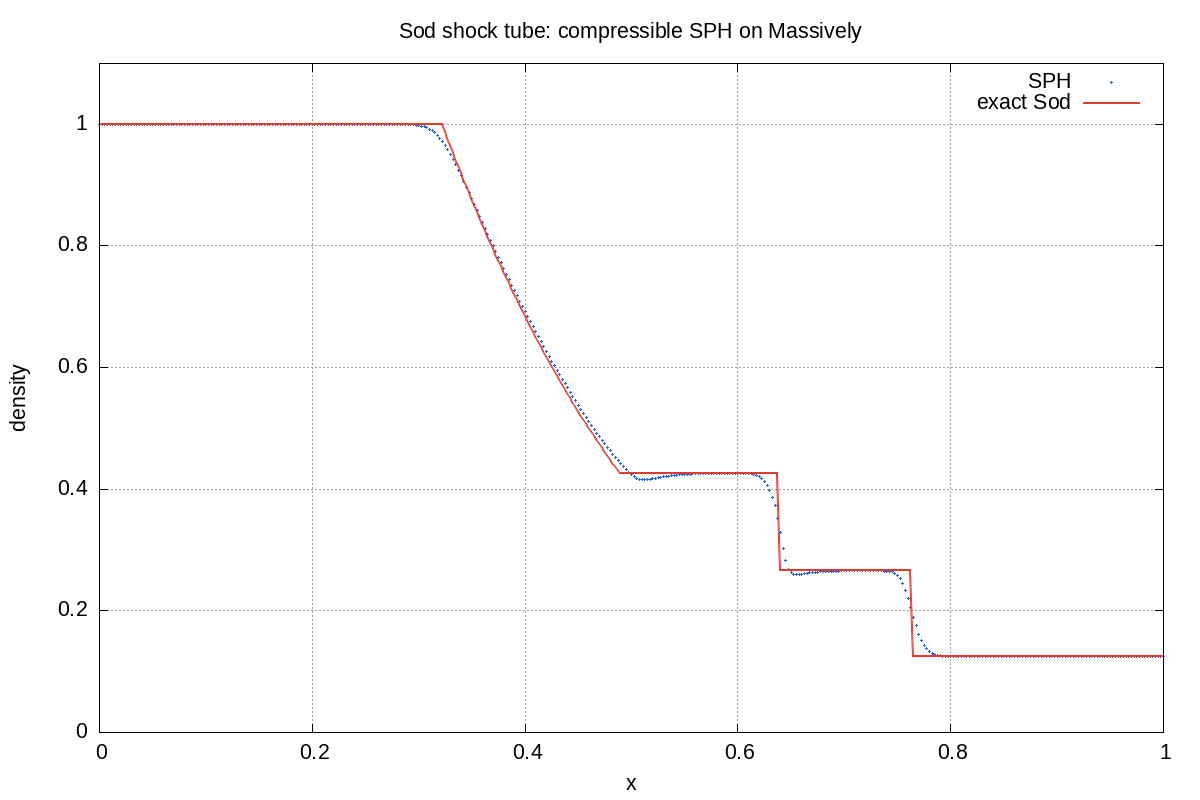
\includegraphics[width=0.88\textwidth]{shocktube.jpeg}
  \caption{Sod shock-tube density.  The GPU SPH solution captures the
  rarefaction, contact discontinuity, and shock at $t=0.15$.}
  \label{fig:shocktube}
\end{figure}

Figure~\ref{fig:shocktube} gives a mean absolute sampled density error of
0.00419917.  The minimum computed density is 0.124903 and the minimum pressure is
0.100179; total particle mass is unchanged.  The exact star state used by the
plot is $p_*=0.303130$ and $u_*=0.927453$.  This result checks the composition of
sorting, density, equation of state, pressure and viscous derivatives, time
integration, and snapshot reconstruction in one evolving problem.  It is not a
convergence study and does not by itself validate every SPH flow regime.

\subsection{Density-pipeline performance}

Benchmarks were run on an AMD Ryzen 7 7735U with an integrated Radeon 680M using
the WGPU backend, Linux 6.17, and Rust 1.96.0.  Reported GPU and CPU cell-list
values are medians of five timed repetitions after warm-up.  The GPU snapshot
includes cell-ID evaluation, sorting, lower-bound construction, nested density,
equation of state, and transfer of the snapshot to the host.  The CPU cell-list
scope includes list construction and density only.  Therefore the two timings
are useful engineering evidence for the neighborhood design, not a
state-of-the-art or full-step solver comparison.

\begin{table}[ht]
  \centering
  \caption{Two-dimensional density benchmark (milliseconds).}
  \label{tab:performance}
  \begin{tabular}{rrrrrr}
    \toprule
    $N$ & GPU snapshot & CPU cells & CPU all pairs & CPU/GPU & max rel. difference \\
    \midrule
     1,024 & 1.976 & 0.247 & 2.876   & 0.125 & $3.12\times10^{-7}$ \\
     4,096 & 2.018 & 0.984 & 44.764  & 0.488 & $1.61\times10^{-6}$ \\
    16,384 & 2.457 & 4.060 & 711.865 & 1.653 & $2.38\times10^{-6}$ \\
    65,536 & 5.109 & 16.204 & ---     & 3.171 & $5.89\times10^{-6}$ \\
    \bottomrule
  \end{tabular}
\end{table}

\begin{figure}[ht]
  \centering
  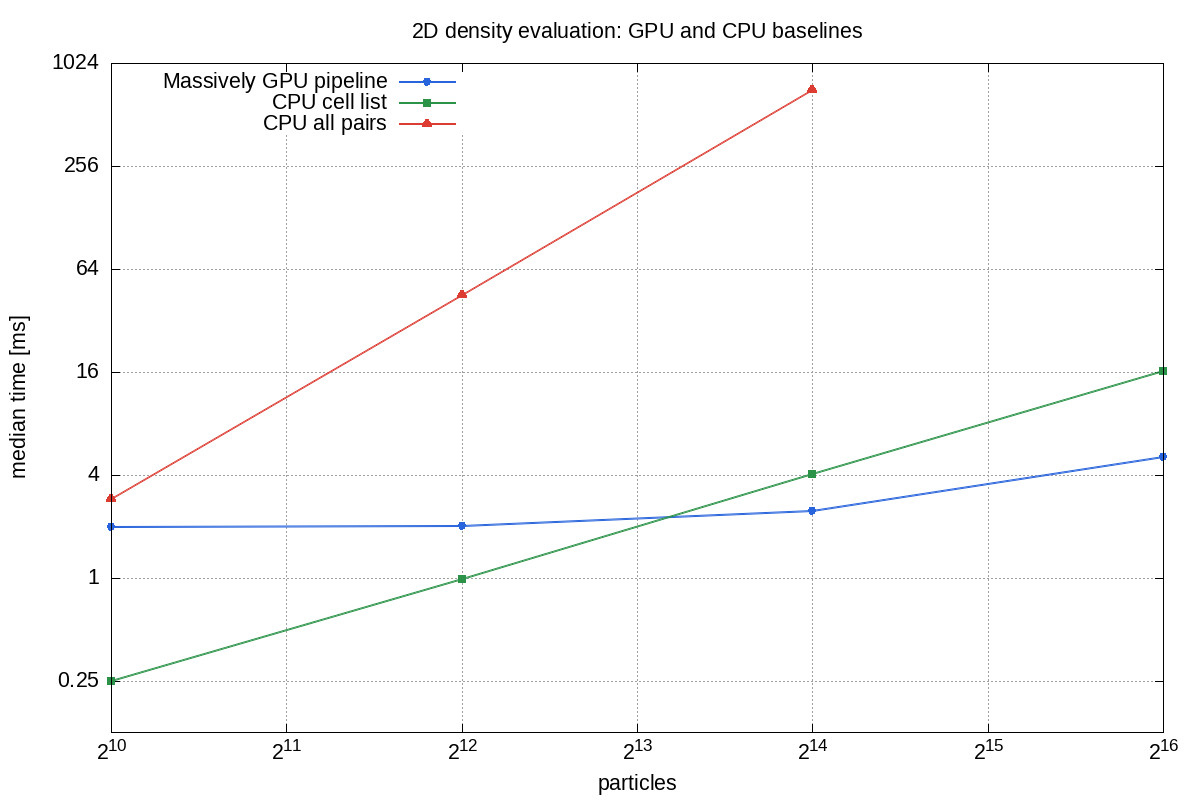
\includegraphics[width=0.96\textwidth]{performance.jpeg}
  \caption{Density-pipeline scaling.  Dispatch overhead dominates small inputs;
  the GPU crosses the CPU cell implementation between 4,096 and 16,384
  particles on the tested machine.}
  \label{fig:performance}
\end{figure}

At 1,024 particles, approximately 2 ms of GPU launch and synchronization cost
makes the host implementation faster.  At 65,536 particles, the GPU snapshot is
3.17 times faster than the CPU cell-list scope despite including equation of
state and host transfer.  At 16,384 particles, CPU all-pairs density is about 290
times slower than the GPU snapshot.  Most importantly for correctness, the
maximum relative difference from the all-pairs density remains
$5.89\times10^{-6}$ at the largest tested size.  These results show that the
nested view lowers to a useful GPU pipeline once enough pair work is available;
they do not identify the sort, pair traversal, or transfer contribution
separately.

\subsection{Reproducibility}

The Cargo lockfile records Massively tag v0.80 at revision
\code{f1041b5cf7902b01c303b2af3f69548e8c05cc91}.  The Rust workspace tests run
with \code{cargo test --workspace}.  Plot scripts and generated JPEG files are
versioned in \code{workspace/draw} and \code{workspace/plot}.  The English and
equivalent Japanese papers are built in the declared Docker environment with
\code{just --justfile paper/justfile}; the outputs are
\code{paper/paper.pdf} and \code{paper/paper-ja.pdf}.

\section{Discussion and limitations}

The key result is representational.  SPH appears to require a mutable graph from
each particle to its neighbors.  In this implementation, only two smaller
relations are stored: a static CSR from cells to neighboring cells and a dynamic
sorted partition from cells to particles.  Nested segmentation and permutation
compute their relational composition at read time.  This is why
\code{SegmentIterator} fits the problem: it carries ragged bounds through a
typed iterator expression without pretending that the neighbor relation is
dense or forcing it to become a separate pair array.

Massively does not make the underlying costs disappear.  The current solver
sorts at every derivative evaluation; a highly nonuniform particle distribution
still causes load imbalance; gather traversal duplicates symmetric pair work;
and the 13-read boundary turns some two-dimensional operators into multiple
dispatches.  These are visible design trade-offs rather than hidden backend
details.

The smoothing length is global and fixed, integration is first-order
symplectic Euler, boundaries are rectangular and reflecting, and the supplied
equation of state is the ideal gas.
The benchmark measures a density snapshot on one integrated GPU, not a complete
long-running simulation across multiple devices.  The Sod result establishes a
credible end-to-end baseline, but resolution sweeps and additional physical
problems would be required to make broader numerical claims.

The most direct implementation-oriented next steps are:
\begin{itemize}
  \item reuse sorted order for substeps in which a displacement bound proves
        that cell membership has not changed;
  \item optionally cache Verlet candidates when the saved traversal work
        outweighs the extra $O(Q)$ storage;
  \item profile sort, lower bound, nested traversal, and transfer independently;
  \item pack vector-valued fields or extend Massively's read arity to reduce the
        number of two-dimensional passes; and
  \item extend the same CSR/segment construction to 3-D, where each row has at
        most 27 cells, and test its occupancy and divergence behavior.
\end{itemize}
Adaptive smoothing length is an important numerical extension, but it also
changes the implementation problem because cell width and per-particle support
can no longer be represented by the present fixed nine-cell stencil without a
conservative support rule.

\section{Conclusion}

The moving SPH neighborhood can be expressed in Massively v0.80 without a
materialized particle-pair list.  The implementation stores a static cell CSR,
sorts all particle columns coherently, derives cell--particle offsets with lower
bounds, and composes both relations through lazy permutation and two nested
\code{SegmentIterator} layers.  Per-query gather transforms avoid atomics, and
separable pre/post passes keep the complete solver within Massively's 13-read
type boundary.  The Sod shock tube checks the evolving solver, differential
density checks the neighborhood against all pairs, and the measured crossover
shows that the representation provides useful GPU throughput.  Equally
important, the design exposes its costs---repeated sorting, duplicated symmetric
work, load imbalance, and extra passes---which gives a concrete basis for the
next round of Massively and SPH implementation work.

{\small
\bibliographystyle{plainnat}
\bibliography{references}
}

\end{document}
